\begin{frame}
  \frametitle{CUDA Generics}
  We talked about generic algorithms, what if we could drop in
  replacement algorithms to take advantage of available hardware?
  \begin{itemize}
    \item What here...
  \end{itemize}
\end{frame}

\begin{frame}[fragile]
  \frametitle{Thrust Namespace}
  Just like the STL is declared inside the \\
  \vspace{.5cm}\hspace{1cm}\lstinline|std|\vspace{.5cm} \\
  namespace, all thrust symbols are declared inside the \\
  \vspace{.5cm}\hspace{1cm}\lstinline|thrust|\vspace{.5cm} \\
  namespace.
\end{frame}

\begin{frame}[fragile]
  \frametitle{Thrust Vectors}
  Device memory is distinct from host memory. We need a special
  container class to refer to device memory:
  \begin{block}{Thrust vector declaration}
    \begin{lstlisting}
    template< typename T >
    class thrust::device_vector<T>;
    \end{lstlisting}
  \end{block}
\end{frame}

\begin{frame}[fragile]
  \frametitle{Thrust Vectors}
  Values can be easily transferred from host to device.
  \begin{example}
    \begin{lstlisting}
    std::vector<float> host_vec( 100 );
    thrust::device_vector<float> dev_vec( 100 );
    thrust::copy( host_vec.begin(), host_vec.end(), dev_vec.begin() );
    \end{lstlisting}
  \end{example}
  Do a bit on noticing I left off the <float> in copy.
\end{frame}

\begin{frame}
  \frametitle{Thrust Algorithms}
  What kinds of algorithms can be optimised for multicore hardware?
  \begin{itemize}
    \item Transformation,
    \item reduction,
    \item sorting,
    \item and others.
  \end{itemize}
\end{frame}

\begin{frame}[fragile]
  \frametitle{Transformation}
  Apply a unary operation to each element of a vector and store the
  result in another (or the same) vector.
  \begin{center}
  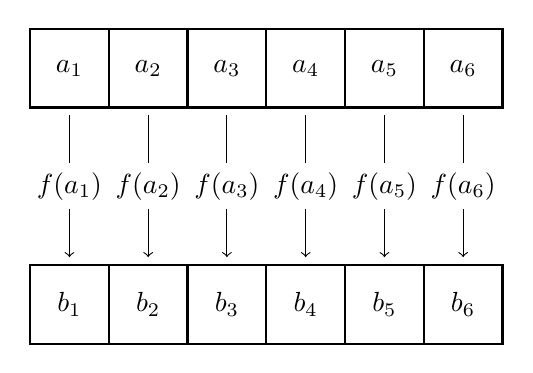
\begin{tikzpicture}[
      box/.style={thick},
      op/.style={rectangle,fill=white},
    ]
    \draw[box] (0,0) rectangle(6,1);
    \draw[box] (0,3) rectangle(6,4);
    \foreach \x in {1,...,6}{
      \draw[box] (\x,0) -- (\x,1);
      \draw[box] (\x,3) -- (\x,4);
      \draw[<-] (\x-.5,1.1) -- (\x-.5,2.9);
      \node at (\x-.5,0.5) {$b_\x$};
      \node at (\x-.5,3.5) {$a_\x$};
      \node[op] at (\x-.5,2) {$f(a_\x)$};
    };
  \end{tikzpicture}
  \end{center}
\end{frame}

\begin{frame}[fragile]
  \frametitle{Reduction}
  Apply a binary operation to successive elements of a vector and return
  the scalar result.
  \begin{center}
  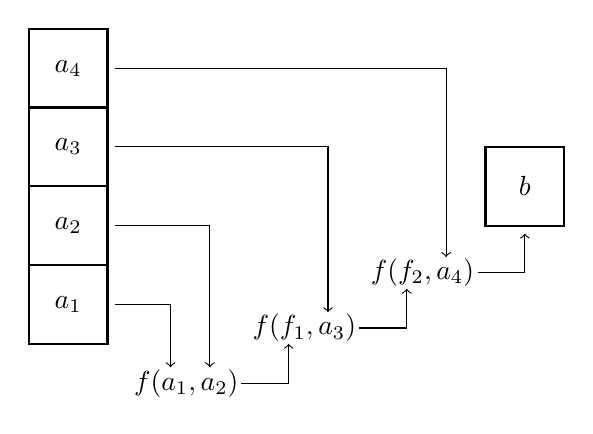
\begin{tikzpicture}[
      box/.style={thick},
      op/.style={rectangle,fill=white},
    ]
    \draw[box] (0,0) rectangle(1,4);
    \foreach \y in {1,...,4}{
      \draw[box] (0,\y) -- (1,\y);
      \node at (.5,\y-.5) {$a_\y$};
    };
    \node at (2,-.5) {$f(a_1,a_2)$};
    \node at (3.5,.2) {$f(f_1,a_3)$};
    \node at (5,.9) {$f(f_2,a_4)$};
    \draw[->] (1.1,.5) -- (1.8,.5) -- (1.8,-.3);
    \draw[->] (1.1,1.5) -- (2.3,1.5) -- (2.3,-.3);
    \draw[->] (1.1,2.5) -- (3.8,2.5) -- (3.8,.4);
    \draw[->] (1.1,3.5) -- (5.3,3.5) -- (5.3,1.1);
    \draw[->] (2.7,-.5) -- (3.3,-.5) -- (3.3,0);
    \draw[->] (4.2,.2) -- (4.8,.2) -- (4.8,.7);
    \draw[->] (5.7,.9) -- (6.3,.9) -- (6.3,1.4);
    \draw[box] (5.8,1.5) rectangle(6.8,2.5);
    \node at (6.3,2) {$b$};
  \end{tikzpicture}
  \end{center}
\end{frame}

\begin{frame}[fragile]
  \frametitle{Sorting}
  Apply an ordering to a vector.
\end{frame}

\begin{frame}
  \frametitle{M}
  Explain that the general operations, transformation and
  reduce, can be applied to a wide range of algorithms.
  Not all, but a wide range. Talk about how the internals of
  these general operations can be modified with functors.
\end{frame}

\begin{frame}[fragile]
  \frametitle{Advanced Iterators}
  Talk a little about \lstinline|constant_iterator|,
  \lstinline|counting_iterator|, \lstinline|transform_iterator| and
  \lstinline|zip_iterator|.
\end{frame}

\begin{frame}
  \frametitle{Examples of Uses}
  List all the different algorithms in the Thrust examples.
\end{frame}
